\documentclass[main]{subfiles}
\newcommand{\todo}[1]{{\color{blue} #1 }}

\begin{document}



\section{Results and discussion}\label{sec:results}


%Single source, 2EqualSizedSource, 4EqualSizedSource, 6EqualSizedSource, 2UnequalSizedSource, 4UnequalSizedSource and 6UnequalSizedSource. The details of the datasets used and the results on individual datasets are given in Supplementary Material.%are given in the following, these data have been taken from the UCI Repository of machine learning batabases: ftp://ftp.ics.uci.edu/pub/machine-learning-databases/.
%
%
%\subsection{Empirical results on Combined data}

\begin{figure}[H]
\centering
\begin{subfigure}{\textwidth}
  \centering
  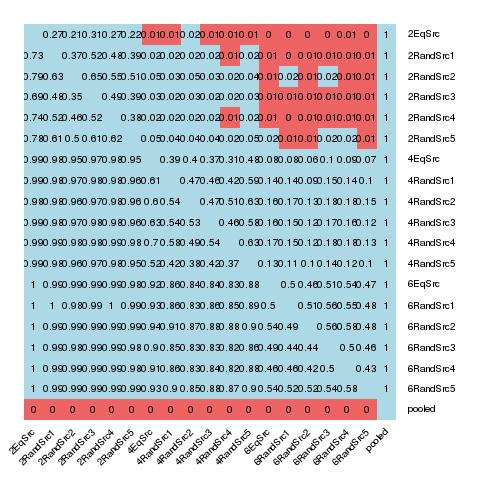
\includegraphics[width=.75\linewidth]{images/heatmapCombined}
%  \caption{Validity}  \label{fig:valCombined}
\end{subfigure}%

\begin{subfigure}{\textwidth}
  \centering
  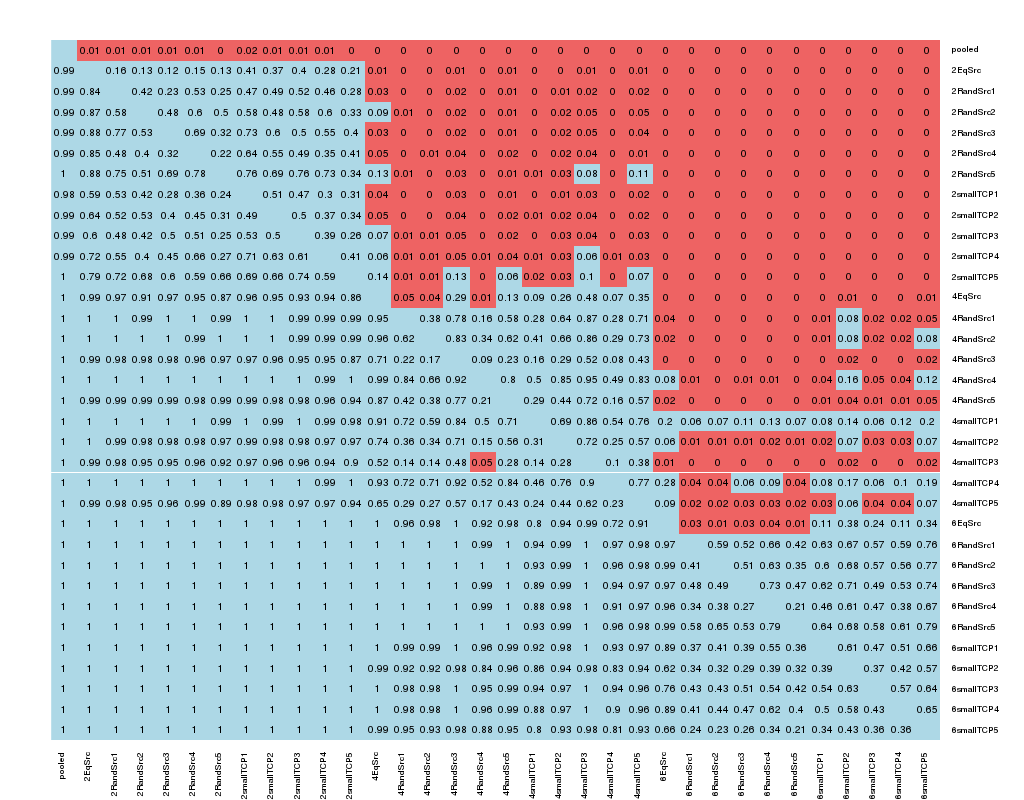
\includegraphics[width=.75\linewidth]{images/heatmapCombined_eff}
  %\caption{Efficiency}  \label{fig:effCombined}
\end{subfigure}%
\caption{Results of Wilcoxon signed-rank tests for two alternative hypotheses relating validity (a) and observed fuzziness (b) with combining all the datasets. The p-values are shown for the scenarios in the right column having greater values than the scenarios in the rows. All significant p-values are marked in red. Pooled: Unpartitioned dataset. EqSrc: equally partitioned data sources, RandSrc: randomly partitioned data sources. smallTCP: a single TCP model.} \label{fig:testCombined}
\end{figure}

%Another figure


\begin{figure}[H]
\begin{center}

%\begin{subfigure}{\textwidth}\centering
%  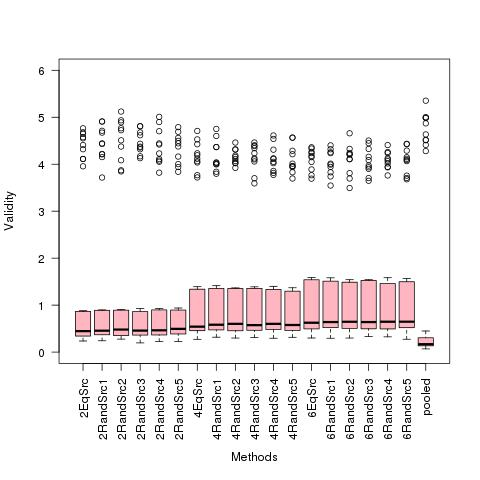
\includegraphics[width=12cm,height=6cm]{images/boxplotCombined}
%  \caption{Validity}  \label{fig:valBC}
%\end{subfigure}%

%\begin{subfigure}{\textwidth} \centering
 
  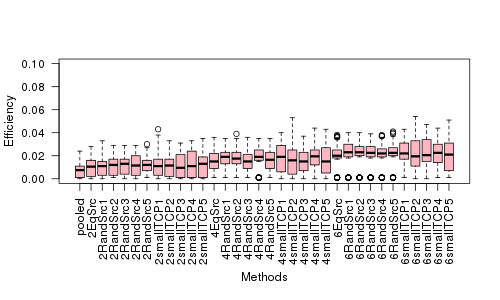
\includegraphics[scale=0.8]{images/boxplotCombined_eff}
 % \caption{Efficiency}  \label{fig:effBC}
%\end{subfigure}%
%\caption{Box plot of validity (a) and observed fuzziness (b) with combined data.}
\caption{Box plot of observed fuzziness for aggregating 0, 2, 4, and 6 non-disclosed data sources. Pooled: Unpartitioned dataset. EqSrc: equally partitioned data sources, RandSrc: randomly partitioned data sources. smallTCP: a single TCP model.}
\label{fig:boxplotCombined}
\end{center}
\end{figure}




%\section{Results and Discussions}
%The aim of this study was to improve predictions over different data sources without explicitly sharing the data, by aggregating conformal predictions computed at individual locations. In order to do so, we investigated if and how the number of data sources and size of these affect the aggregated efficiency and validity.
The results from the pairwise comparison of validity and efficiency (observed fuzziness) are shown in Figure \ref{fig:testCombined}. To illustrate the quantitative difference between the scenarios, box plots are presented in Figure~\ref{fig:boxplotCombined}.
%
Results in Figure~\ref{fig:testCombined} show that pooled is significantly more efficient than all other models, as would be expected, but in absolute numbers the decrease in efficiency is not so large when using NDCP. When comparing NDCP with individual smallTCP, we do not see a significant improvement in efficiency using NDCP but we observe a reduced variance, consistent with previous work~\citep{Carlsson:2014qr}, when there are 4 or more partitions. We also observe in Figure~\ref{fig:testCombined} that there is no significant difference between 'aggregated equally partitioned' and 'aggregated randomly partitioned', which would make the method generally applicable regardless of the sizes of individual training sets.

%NDCP more efficient predictions than individual analyses
%1. To investigate if and how the number of data sources and size of the sources affect the aggregated efficiency and validity

%\subsection{Validity}
Regarding validity, we observe that the pooled model is always valid, as an example see Figure~\ref{fig:pooledCalibrationPlot} for the Spambase dataset. Further, we see that individual small models are also valid, see Figure~\ref{fig:valIndividual} for randomly partitioned small TCPs for Spambase dataset. Consistent with previous work by Linusson et al~\cite{Linusson:2017dn} and Carlsson et al.~\cite{Carlsson:2014qr}, NDCP is less valid overall, see Figure~\ref{fig:valCombined} for randomly partitioned NDCPs for Spambase dataset, but calibration plot shows conservative validity for the significance levels 0 to 0.5 which is the interesting region for predictions. This is a known issue that requires further research; we settle here with the observation that validity does not seem to be a practical problem for NDCP in the interesting significance region.

\begin{figure}[H]
\begin{center}
  \begin{subfigure}{.3\textwidth}
  \centering
  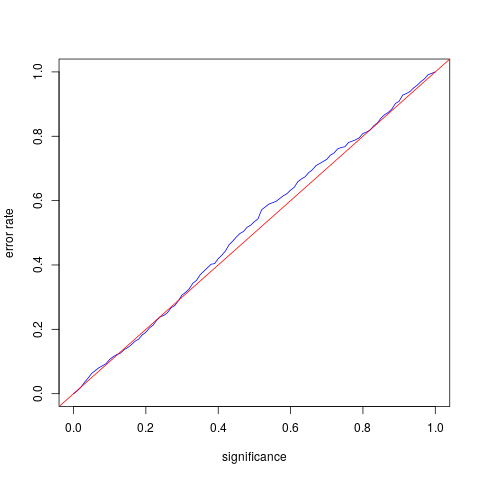
\includegraphics[scale=0.2]{images/pooledCalibrationPlot}
  \caption{pooled} \label{fig:pooledCalibrationPlot}
   \end{subfigure}    
  \begin{subfigure}{.3\textwidth}
  \centering
  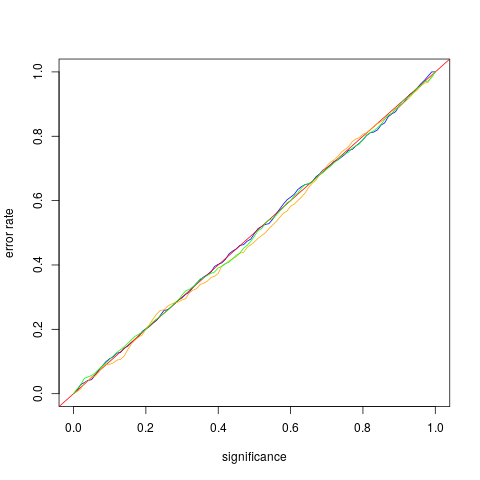
\includegraphics[scale=0.2]{images/eqSourceInd}
  \caption{smallTCPs}\label{fig:valIndividual}
  \end{subfigure}
  \begin{subfigure}{.3\textwidth}
  \centering
  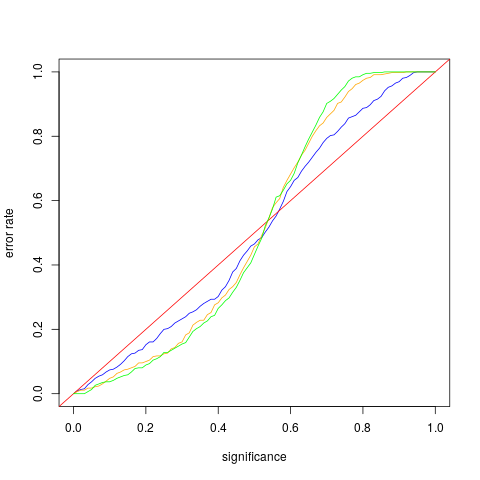
\includegraphics[scale=0.2]{images/eqSourceCombined}
  \caption{NDCPs}\label{fig:valCombined}
  \end{subfigure}
  
 \caption{Calibration plot for various models. a) Calibration plot of TCP for one fold of Spambase dataset. b) Calibration plot of randomly partitioned small TCPs for one fold of  Spambase dataset. Blue, orange and  green line indicate each small TCP from two, four and six source random partitions respectively. c) Calibration plot of NDCPs for one fold of Spambase dataset. Blue, orange and  green line indicate NDCP from two, four and six source random partitions respectively}
 
\end{center}
\end{figure}


%\subsection{Efficiency}
%2. to evaluate how good both aggregated equally partitioned and aggregated randomly partitioned perform when compared to the whole (pooled) data set.


%3. to evaluate if and under what conditions unbalanced aggregated TCP delivers acceptable results when compared to pooled data





\section{Conclusions}
We present a method to aggregate conformal predictions from multiple sources while preserving data privacy. The method is a generalization of the basic conformal prediction framework to handle multiple data sources without disclosing data between the data sources. Due to its low complexity for implementation, we believe the method will be useful for organizations that wish to make predictions over combined data without disclosing data to each other, such as for drug discovery problems when pharmaceutical companies wishes to establish predictive models of drug safety.




\end{document}



